\documentclass[10pt]{beamer}

\usetheme[progressbar=frametitle]{metropolis}
\usepackage{appendixnumberbeamer}

\usepackage{booktabs}
\usepackage[scale=2]{ccicons}

\usepackage{pgfplots}
\usepgfplotslibrary{dateplot}

\usepackage{xspace}
\newcommand{\themename}{\textbf{\textsc{metropolis}}\xspace}

\usepackage{graphicx}
\graphicspath{ {pics/} }

\usepackage{listings}
\definecolor{mGreen}{rgb}{0,0.6,0}
\definecolor{mGray}{rgb}{0.5,0.5,0.5}
\definecolor{mPurple}{rgb}{0.58,0,0.82}
\definecolor{backgroundColour}{rgb}{0.95,0.95,0.92}

\lstdefinestyle{CStyle}{
    backgroundcolor=\color{backgroundColour},   
    commentstyle=\color{mGreen},
    keywordstyle=\color{magenta},
    numberstyle=\tiny\color{mGray},
    stringstyle=\color{mPurple},
    basicstyle=\footnotesize,
    breakatwhitespace=false,         
    %breaklines=true,                 
    captionpos=b,                    
    keepspaces=true,                 
    %numbers=left,                    
    numbersep=5pt,                  
    showspaces=false,                
    showstringspaces=false,
    showtabs=false,                  
    tabsize=2,
    language=C
}

%----------------------------------------------------------------------------------------
%	TITLE PAGE
%----------------------------------------------------------------------------------------

\title{Netze und Verteilte Systeme}
\subtitle{Programmierprojekt}
% \date{\today}
\date{}
\author{Dmitrii Polianskii, Lukas Lamminger}
\institute{Universit\"at Salzburg}
% \titlegraphic{\hfill\includegraphics[height=1.5cm]{logo.pdf}}

\begin{document}

\maketitle

% \begin{frame}{Themen}
%   \setbeamertemplate{section in toc}[sections numbered]
%   \tableofcontents[hideallsubsections]
% \end{frame}

%----------------------------------------------------------------------------------------
%	Einleitung
%----------------------------------------------------------------------------------------


\begin{frame}[fragile]{Usage TX}
	\begin{block}{C:}
		\hspace*{2mm} \footnotesize 	 ./TX portTX portRX packet\_size packet\_block\_size send\_delay file\_name
	\end{block}

	\begin{block}{java:}
		\hspace*{2mm} \footnotesize 	 java TX portTX portRX packet\_size packet\_block\_size send\_delay file\_name
	\end{block}
		
  \begin{itemize}
  	\footnotesize 	
    \item{\textbf{portTX}} - port to recieve acknowlegments (default: 4700)
    \item{\textbf{portRX}} - port to send datagrams (default: 4711)
    \item{\textbf{packet\_size}} - size of a packet in Bytes (default: 1000)
    \item{\textbf{packet\_block\_size}} - amount of packets between delay (default: 100)
    \item{\textbf{send\_delay}} - delay in microsec between blocks (default: 200)
    \item{\textbf{file\_name}} - name of a file to transmit (default: to\_send.jpg)
  \end{itemize}
\end{frame}

\begin{frame}[fragile]{Usage RX}
	\begin{block}{C:}
		\hspace*{2mm} \footnotesize ./RX portTX portRX 
	\end{block}

	\begin{block}{java:}
		\hspace*{2mm} \footnotesize java portRX portRX 
	\end{block}
		
  \begin{itemize}
  	\footnotesize 	
    \item{\textbf{portTX}} - port to send acknowlegments (default: 4700)
    \item{\textbf{portRX}} - port to recieve datagrams (default: 4711)
  \end{itemize}
\end{frame}

\begin{frame}[fragile]{Header structure}

  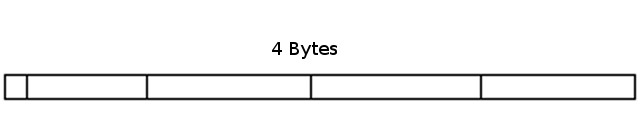
\includegraphics[width=\linewidth]{header}
  \newline
  A header consists of 4 bytes. 
  \newline
  First bit is used to indicate the last packet. 
  \newline
  31 bits left for sequence number

\end{frame}


\begin{frame}[fragile]{TX description}
	\begin{block}{TX description}
		\begin{enumerate}
		\item Read file
		\begin{enumerate}
			\item Read file in buffer
			\item Calculate CRC32 and add to filebytes
			\item Split filebytes in packages
		\end{enumerate}
		\item Initialize UPD Socket
		\item Initialize Acknowlegments array to obtain transmitted packets
		\item Transmit one block of packets
		\begin{enumerate}
			\item For every packet in block check if acknolegment was recieved, if not - send a packet.
			\item If last packet is reached, then start with first again,
		\end{enumerate}
		\item Wait for acknowlegments \{DELAY\} microseconds.
		\begin{enumerate}
			\item Write every sequence number from acknowlegment packet in Acknowlegments array,
			\item If all packets were acknowlegment - end transmission. Else - goto punkt 4.
		\end{enumerate}
		\end{enumerate}
	\end{block}
\end{frame}




\begin{frame}[fragile]{RX description}
	\begin{block}{RX description}
		\begin{enumerate}
		\item Initialize UPD Socket
		\item Listen for incomming packages
		\begin{enumerate}
			\item Write databits from package in a memory
			\item If last-package-bit was seen, the size of file and Amount of packets can be defined.
			\item If not all of package were recieved, then goto punkt 2.
		\end{enumerate}
		\item Assemble a file
		\item Calculate CRC32 and compare with recieved one.
		\end{enumerate}
	\end{block}
\end{frame}


\end{document}
